
\providecommand{\Cat}{\mathcal{C}at}

\section{2-\trCategory{}论概念的可表示刻画}\label{sec:representable-characterizations}

在由 2-\trCategory{}组成的\trCartesianClosed{}\trCategory{}中，伴随任何%
2-\trCategory{} $\mathcal{C}$ 的 hom 2-\trFunctor{}
$\mathcal{C}(-,-)\colon\mathcal{C}^{\mathrm{op}}\times\mathcal{C}\to\Cat$
经转置便定义一支 \trYonedaEmbedding{} 2-\trFunctor{}
$\flat\colon\mathcal{C}\hookrightarrow\Cat^{\mathcal{C}^{\mathrm{op}}}$；余定义域则为
由从 $\mathcal{C}$ 到 $\Cat$ 的那些 2-\trFunctor、2-\trNaturalTransformation{}与%
\trModification{}组成的 2-\trCategory。由富集 \trYonedaLemma，这支 2-\trFunctor{}在富集
意义下是\trFullyFaithful：2-\trCategory{} $\mathcal{C}$ 同构于由诸可表示%
2-\trFunctor{} $\mathcal{C}(-,x)\colon\mathcal{C}^{\mathrm{op}}\to\Cat$ 张成的
满子 2-\trCategory。鉴于这一富集全忠实性，诸如\trEquivalence{}或%
\trAdjunction{}这类在 2-\trCategory{} $\mathcal{C}$ 内部定义的结构，皆为该%
\trYonedaEmbedding{}所既保持又反射。

这个结果并不如人们所期待的那般有用。事实上，本节所证明的关于%
\trEquivalence、\trAdjunction{}与绝对\trLifting{}图的种种「可表示刻画」没有
一个是它的推论。要点在于，$\Cat^{\mathcal{C}}$ 中的诸 1-\trCell{}是%
2-\trNaturalTransformation，但正如我们的证明所揭示的，更弱的自然性条件已足以
检出 $\mathcal{C}$ 中存在的那些 2-范畴结构。

关于 Yoneda 观点，我们将在本节末尾的\cref{rem:yoneda-perspective}中多说几句。

与第 1 章中的\cref{thm:equivalences-are-equivalences}相类比，我们有如下结果，
它告诉我们：一个 2-\trCategory{}中的诸\trEquivalence{}表示诸\trCategory{}的%
\trEquivalence。

\begin{proposition}[\trEquivalence{}是可表示地定义的]\label{prop:equivalences-representably-defined}
2-\trCategory{} $\mathcal{C}$ 中的一支 1-\trCell{} $f\colon a\to b$ 定义一个%
\trEquivalence，当且仅当对一切 $x\in\mathcal{C}$，其所诱导的\trFunctor
\[
\mathcal{C}(x,a)\xrightarrow{\;f_{\ast}\;}\mathcal{C}(x,b)
\]
定义诸\trCategory{}的一个\trEquivalence。
\end{proposition}

\begin{proof}
每个 $x\in\mathcal{C}$ 都定义一支 2-\trFunctor{}
$\mathcal{C}(x,-)\colon\mathcal{C}\to\Cat$，于是若 $f\colon a\Rightarrow b$
是 $\mathcal{C}$ 中的一个\trEquivalence，则
$f_{\ast}\colon\mathcal{C}(x,a)\Rightarrow\mathcal{C}(x,b)$ 是 $\Cat$ 中的
一个\trEquivalence。

反之，由 $f_{\ast}\colon\mathcal{C}(b,a)\Rightarrow\mathcal{C}(b,b)$ 的本质满性，
存在某支 $g\colon b\to a$ 与一个\trIsomorphism{} $\beta\colon fg\cong\mathrm{id}_{b}$。
由 $f_{\ast}\colon\mathcal{C}(a,a)\Rightarrow\mathcal{C}(a,b)$ 的全忠实性，%
\trIsomorphism{} $\beta^{-1}f\colon f\cong fgf$ 可提升为一个\trIsomorphism{}
$\alpha\colon\mathrm{id}_{a}\cong gf$。
\end{proof}

类似地，2-\trCategory{}中的一支\trAdjunction{}\trFunctor{}在诸 \trHomCategory{}%
之间诱导逐点定义的\trAdjunction，但在此情形下，还需要一个进一步的「正合性」
条件，才能把一个可表示地定义的\trAdjunction{}转化为该 2-\trCategory{}中的
一个\trAdjunction。

\begin{proposition}[\trAdjunction{}是可表示地定义的]\label{prop:adjunctions-representably-defined}
2-\trCategory{} $\mathcal{C}$ 中的一支 1-\trCell{} $u\colon a\to b$ 容许
一个\trLeftAdjoint，当且仅当：
\begin{enumerate}[label=(\roman*)]
\item 对一切 $x\in\mathcal{C}$，所诱导的\trFunctor{}容许一个\trLeftAdjoint
\begin{center}
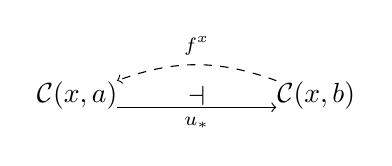
\begin{tikzpicture}[x=1.6em,y=1.2em]
  \node (xa) at (0,0) {$\mathcal{C}(x,a)$};
  \node (xb) at (5.4,0) {$\mathcal{C}(x,b)$};
  \draw[->,dashed] (4.5,0.45) to[bend right=20]
    node[above]{$\scriptstyle f^{x}$} (0.9,0.45);
  \node at (2.7,0) {$\dashv$};
  \draw[->] (0.9,-0.35) -- node[below]{$\scriptstyle u_{\ast}$} (4.5,-0.35);
\end{tikzpicture}
\end{center}
\item 对一切 $k\colon y\to x\in\mathcal{C}$，恒等 2-\trCell{}的\trMate{}是一个%
\trIsomorphism：
\begin{center}
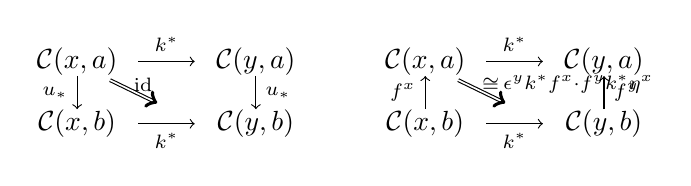
\begin{tikzpicture}[x=1.7em,y=1.5em]
  \node (xa1) at (0,1.5) {$\mathcal{C}(x,a)$};
  \node (ya1) at (3.8,1.5) {$\mathcal{C}(y,a)$};
  \node (xb1) at (0,0) {$\mathcal{C}(x,b)$};
  \node (yb1) at (3.8,0) {$\mathcal{C}(y,b)$};
  \draw[->] (1.3,1.5) -- node[above]{$\scriptstyle k^{\ast}$} (2.5,1.5);
  \draw[->] (1.3,0) -- node[below]{$\scriptstyle k^{\ast}$} (2.5,0);
  \draw[->] (0,1.15) -- node[left]{$\scriptstyle u_{\ast}$} (0,0.35);
  \draw[->] (3.8,1.15) -- node[right]{$\scriptstyle u_{\ast}$} (3.8,0.35);
  \draw[->,double] (0.7,1.05) -- (1.7,0.5);
  \node[right] at (1.0,0.95) {$\scriptstyle\mathrm{id}$};
  \node at (5.6,0.75) {$\rightsquigarrow$};
  \node (xa2) at (7.4,1.5) {$\mathcal{C}(x,a)$};
  \node (ya2) at (11.2,1.5) {$\mathcal{C}(y,a)$};
  \node (xb2) at (7.4,0) {$\mathcal{C}(x,b)$};
  \node (yb2) at (11.2,0) {$\mathcal{C}(y,b)$};
  \draw[->] (8.7,1.5) -- node[above]{$\scriptstyle k^{\ast}$} (9.9,1.5);
  \draw[->] (8.7,0) -- node[below]{$\scriptstyle k^{\ast}$} (9.9,0);
  \draw[->] (7.4,0.35) -- node[left]{$\scriptstyle f^{x}$} (7.4,1.15);
  \draw[->] (11.2,0.35) -- node[right]{$\scriptstyle f^{y}$} (11.2,1.15);
  \draw[->,double] (8.1,1.05) -- (9.1,0.5);
  \node[right] at (8.4,0.95)
    {$\scriptstyle\cong\,\epsilon^{y}k^{\ast}f^{x}\cdot f^{y}k^{\ast}\eta^{x}$};
\end{tikzpicture}
\end{center}
\end{enumerate}
\end{proposition}

\begin{proof}
\trYonedaEmbedding{} 2-\trFunctor{}
$\flat\colon\mathcal{C}\hookrightarrow\Cat^{\mathcal{C}^{\mathrm{op}}}$ 保持诸%
\trAdjunction，把 $\mathcal{C}$ 中的一个\trAdjunction{}对 $f\dashv u$ 携带为
诸可表示 2-\trFunctor{} $\mathcal{C}(-,a)$ 与 $\mathcal{C}(-,b)$ 之间的一个%
\trAdjunction
\begin{center}
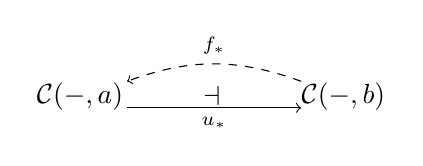
\begin{tikzpicture}[x=1.7em,y=1.2em]
  \node (ma) at (0,0) {$\mathcal{C}(-,a)$};
  \node (mb) at (5.6,0) {$\mathcal{C}(-,b)$};
  \draw[->,dashed] (4.7,0.45) to[bend right=20]
    node[above]{$\scriptstyle f_{\ast}$} (1.0,0.45);
  \node at (2.8,0) {$\dashv$};
  \draw[->] (1.0,-0.35) -- node[below]{$\scriptstyle u_{\ast}$} (4.7,-0.35);
\end{tikzpicture}
\end{center}
其左与右伴随是 2-\trNaturalTransformation{} $f_{\ast}\dashv u_{\ast}$，而其%
\trUnit{}与\trCounit{}则是\trModification{}。在 $x\in\mathcal{C}$ 处求值，这便定义出如%
\cref{prop:adjunctions-representably-defined}(i)所示的一族\trAdjunction{}以及%
\textbf{严格伴随态射}（strict adjunction morphisms），意即：任何
$k\colon y\to x$ 就左、右伴随而言都诱导一个严格交换的方块，其中栖居着一对为
恒等 2-\trCell{}的\trMate{}。

真正的内容在逆命题之中。假定 (i)，定义候选的左逆
$f\coloneqq f^{b}(\mathrm{id}_{b})$。由构造
$uf\coloneqq u_{\ast}f^{b}(\mathrm{id}_{b})$，故我们可以把候选的\trUnit{}取为
$f^{b}\dashv u_{\ast}$ 的\trUnit{} $\eta^{b}$ 在 $\mathrm{id}_{b}$ 处的分量：
\[
\eta\coloneqq\mathrm{id}_{b}\;\overset{\eta^{b}_{\mathrm{id}_{b}}}{\Longrightarrow}\;uf
\qquad\in\mathcal{C}(b,b).
\]
注意到这些定义并不先验地给出关于另一复合 $fu\in\mathcal{C}(a,a)$ 的任何信息，
但条件 (ii) 定义了一个自然\trIsomorphism{} $\alpha\colon f^{a}u^{\ast}\cong u^{\ast}f^{b}$
\begin{center}
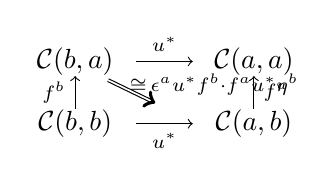
\begin{tikzpicture}[x=1.7em,y=1.5em]
  \node (sa) at (0,1.5) {$\mathcal{C}(b,a)$};
  \node (sb) at (3.8,1.5) {$\mathcal{C}(a,a)$};
  \node (sc) at (0,0) {$\mathcal{C}(b,b)$};
  \node (sd) at (3.8,0) {$\mathcal{C}(a,b)$};
  \draw[->] (1.3,1.5) -- node[above]{$\scriptstyle u^{\ast}$} (2.5,1.5);
  \draw[->] (1.3,0) -- node[below]{$\scriptstyle u^{\ast}$} (2.5,0);
  \draw[->] (0,0.35) -- node[left]{$\scriptstyle f^{b}$} (0,1.15);
  \draw[->] (3.8,0.35) -- node[right]{$\scriptstyle f^{a}$} (3.8,1.15);
  \draw[->,double] (0.7,1.05) -- (1.7,0.5);
  \node[right] at (0.95,0.95)
    {$\scriptstyle\cong\,\epsilon^{a}u^{\ast}f^{b}\cdot f^{a}u^{\ast}\eta^{b}$};
\end{tikzpicture}
\end{center}
其在 $\mathrm{id}_{b}$ 处的分量定义一个\trIsomorphism
\[
\alpha_{\mathrm{id}_{b}}\coloneqq f^{a}(u)\;
\overset{f^{a}(\eta u)}{\Longrightarrow}\;f^{a}(ufu)=f^{a}u_{\ast}(fu)\;
\overset{\epsilon^{a}(fu)}{\Longrightarrow}\;fu
\qquad\in\mathcal{C}(a,a).
\]
据此，我们把\trCounit{}定义为这个\trIsomorphism{}之逆与 $f^{a}\dashv u_{\ast}$
的\trCounit{} $\epsilon^{a}$ 在 $\mathrm{id}_{a}$ 处的分量之复合：
\[
\epsilon\coloneqq fu\;
\underset{\cong}{\overset{\alpha^{-1}_{\mathrm{id}_{b}}}{\Longrightarrow}}\;f^{a}(u)\;
\overset{\epsilon^{a}_{\mathrm{id}_{a}}}{\Longrightarrow}\;\mathrm{id}_{a}
\qquad\in\mathcal{C}(a,a).
\]
交换图
\begin{center}
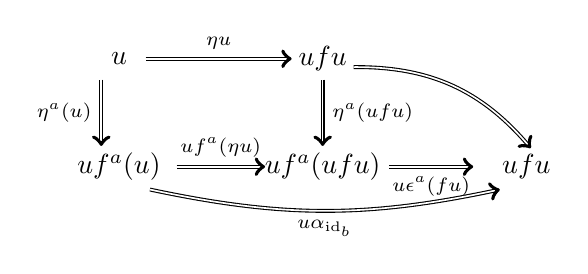
\begin{tikzpicture}[x=1.6em,y=1.5em]
  \node (u)   at (0,2.6)    {$u$};
  \node (ufu) at (4.6,2.6)  {$ufu$};
  \node (ufau)   at (0,0)   {$uf^{a}(u)$};
  \node (ufaufu) at (4.6,0) {$uf^{a}(ufu)$};
  \node (ufu2) at (9.2,0)   {$ufu$};
  \draw[->,double] (0.6,2.6) -- node[above]{$\scriptstyle\eta u$} (3.9,2.6);
  \draw[->,double] (-0.4,2.1) -- node[left]{$\scriptstyle\eta^{a}(u)$} (-0.4,0.5);
  \draw[->,double] (4.6,2.1) -- node[right]{$\scriptstyle\eta^{a}(ufu)$} (4.6,0.5);
  \draw[->,double] (1.3,0) -- node[above]{$\scriptstyle u f^{a}(\eta u)$} (3.3,0);
  \draw[->,double] (6.1,0) -- node[below]{$\scriptstyle u\epsilon^{a}(fu)$} (8.0,0);
  \draw[->,double] (5.3,2.4) to[bend left=25] (9.3,0.45);
  \draw[->,double] (0.7,-0.55) to[bend right=12]
    node[below]{$\scriptstyle u\alpha_{\mathrm{id}_{b}}$} (8.6,-0.55);
\end{tikzpicture}
\end{center}
揭示出 $u\alpha_{\mathrm{id}_{b}}\cdot\eta^{a}u=\eta u$，于是
\[
u\epsilon\cdot\eta u
=(u\epsilon^{a}_{\mathrm{id}_{a}}\cdot u\alpha^{-1}_{\mathrm{id}_{b}})
 \cdot(u\alpha_{\mathrm{id}_{b}}\cdot\eta^{a}u)
=u\epsilon^{a}_{\mathrm{id}_{a}}\cdot\eta^{a}u
=\mathrm{id}_{u},
\]
这便验证了两个\trTriangleEqualities{}中的一个。%
\footnote{原书印作「$u\epsilon^{a}_{\mathrm{id}_{a}}\cdot u\alpha_{\mathrm{id}_{b}}=\mathrm{id}_{u}$」。按前一步之展开，
$u\alpha^{-1}_{\mathrm{id}_{b}}$ 与 $u\alpha_{\mathrm{id}_{b}}$ 应相消，第三段
当为 $u\epsilon^{a}_{\mathrm{id}_{a}}\cdot\eta^{a}u$（末步即由
$f^{a}\dashv u_{\ast}$ 的\trTriangleEqualities{}给出），所印
$u\alpha_{\mathrm{id}_{b}}$ 处数学不通，疑为排印之误，此处径改。——译者注}
要证明另一个\trTriangleEqualities{}的复合
\[
f\;\overset{\eta}{\Longrightarrow}\;fuf\;\overset{\epsilon}{\Longrightarrow}\;f
\qquad\in\mathcal{C}(b,a)
\]
是恒等的，则有些微妙，因为我们没有任何办法理解箭头 $f\eta$。然而注意到，这个
箭头定义了对象 $f^{b}(\mathrm{id}_{b})\in\mathcal{C}(b,a)$ 的一个自同态，于是
如果我们验证：它在\trAdjunction{} $f^{b}\dashv u_{\ast}$ 下的转置是\trUnit{}%
分量 $\eta^{b}_{\mathrm{id}_{b}}$，那么由伴随转置的唯一性，必有
$\epsilon f\cdot f\eta=\mathrm{id}_{f}$，正如所愿。这可以通过直接计算来验证：
伴随转置的计算方法是先作用\trFunctor{} $u_{\ast}$、再与
$\eta^{b}_{\mathrm{id}_{b}}=\eta$ 作预复合，这便给出下图的左下复合：
\begin{center}
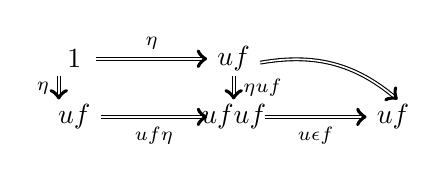
\begin{tikzpicture}[x=1.6em,y=1.4em]
  \node (one) at (0,1.5)  {$1$};
  \node (uft)  at (3.6,1.5) {$uf$};
  \node (ufb)  at (0,0)   {$uf$};
  \node (ufuf) at (3.6,0) {$ufuf$};
  \node (ufbr) at (7.2,0) {$uf$};
  \draw[->,double] (0.5,1.5) -- node[above]{$\scriptstyle\eta$} (3.0,1.5);
  \draw[->,double] (-0.35,1.05) -- node[left]{$\scriptstyle\eta$} (-0.35,0.45);
  \draw[->,double] (3.6,1.05) -- node[right]{$\scriptstyle\eta uf$} (3.6,0.45);
  \draw[->,double] (0.6,0) -- node[below]{$\scriptstyle uf\eta$} (3.0,0);
  \draw[->,double] (4.3,0) -- node[below]{$\scriptstyle u\epsilon f$} (6.6,0);
  \draw[->,double] (4.2,1.4) to[bend left=25] (7.3,0.45);
\end{tikzpicture}
\end{center}
一次利用了先前验证过的\trTriangleEqualities{}的简单追图便完成了证明。
\end{proof}

\cref{prop:adjunctions-representably-defined}的条件 (ii) 被称为一个
「Beck--Chevalley」条件或\emph{正合性}条件。另一个正合性条件出现在绝对%
\trLifting{}图的一个可表示刻画之中。

\begin{definition}\label{def:right-exact-transformation}
介于如下所示的一对绝对右\trLifting{}图 $(r,\rho)$ 与 $(r',\rho')$ 之间的一个%
\trFunctor{}三元组 $(u,v,w)$ 定义一个\textbf{右正合变换}（right exact
transformation），当且仅当由绝对右\trLifting{}的\trUniversalProperty{}所诱导
的 2-\trCell{} $\tau$ 是\trInvertible：
\begin{rveq}\label{eq:right-exact-diagrams}
\mbox{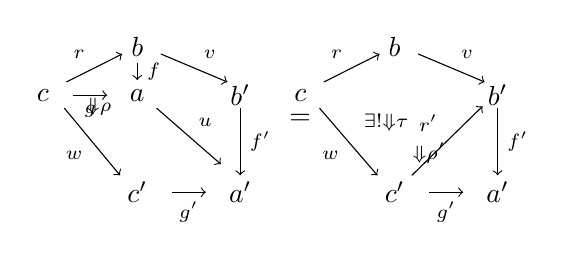
\begin{tikzpicture}[x=1.55em,y=1.35em]
  \node (lb)  at (2.2,2.6)  {$b$};
  \node (lc)  at (0,1.3)    {$c$};
  \node (la)  at (2.2,1.3)  {$a$};
  \node (lbp) at (4.6,1.3)  {$b'$};
  \node (lcp) at (2.2,-1.3) {$c'$};
  \node (lap) at (4.6,-1.3) {$a'$};
  \draw[->] (0.55,1.65) -- node[above left]{$\scriptstyle r$} (1.85,2.4);
  \draw[->] (2.2,2.15) -- node[right]{$\scriptstyle f$} (2.2,1.7);
  \draw[->] (2.75,2.4) -- node[above right]{$\scriptstyle v$} (4.3,1.65);
  \node at (1.3,1.0) {$\scriptstyle\Downarrow\rho$};
  \draw[->] (0.7,1.3) -- node[below]{$\scriptstyle g$} (1.5,1.3);
  \draw[->] (0.5,0.95) -- node[below left]{$\scriptstyle w$} (1.8,-0.85);
  \draw[->] (2.65,0.95) -- node[above right]{$\scriptstyle u$} (4.15,-0.55);
  \draw[->] (4.6,0.95) -- node[right]{$\scriptstyle f'$} (4.6,-0.85);
  \draw[->] (3.0,-1.3) -- node[below]{$\scriptstyle g'$} (3.8,-1.3);
  \node at (6.0,0.65) {$=$};
  \node (rb)  at (8.2,2.6)  {$b$};
  \node (rc)  at (6.0,1.3)  {$c$};
  \node (rbp) at (10.6,1.3) {$b'$};
  \node (rcp) at (8.2,-1.3) {$c'$};
  \node (rap) at (10.6,-1.3) {$a'$};
  \draw[->] (6.55,1.65) -- node[above left]{$\scriptstyle r$} (7.85,2.4);
  \draw[->] (8.75,2.4) -- node[above right]{$\scriptstyle v$} (10.3,1.65);
  \draw[->] (6.45,0.95) -- node[below left]{$\scriptstyle w$} (7.8,-0.85);
  \draw[->] (8.6,-0.85) -- node[above left]{$\scriptstyle r'$} (10.25,1.0);
  \node at (9.0,-0.25) {$\scriptstyle\Downarrow\rho'$};
  \draw[->] (10.6,0.95) -- node[right]{$\scriptstyle f'$} (10.6,-0.85);
  \draw[->] (9.0,-1.3) -- node[below]{$\scriptstyle g'$} (9.8,-1.3);
  \node at (8.0,0.55) {$\scriptstyle\exists!\Downarrow\tau$};
\end{tikzpicture}}
\end{rveq}
\end{definition}

这个右正合性条件成立，当且仅当在 \eqref{eq:right-exact-diagrams} 左侧的图中，
经须化的 2-\trCell{} $u\rho$ 展示 $vr$ 为
$g'w$ 沿 $f'$ 的绝对右\trLifting{}——也就是说，右正合变换正是保持绝对右%
\trLifting{}图的那些变换。

\begin{lemma}\label{lem:mate-right-exact}
如下左伴随之间的交换方图
\begin{center}
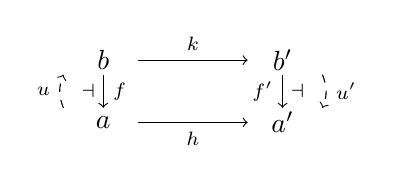
\begin{tikzpicture}[x=1.8em,y=1.5em]
  \node (b)  at (1.8,1.5) {$b$};
  \node (bp) at (5.4,1.5) {$b'$};
  \node (a)  at (1.8,0)   {$a$};
  \node (ap) at (5.4,0)   {$a'$};
  \draw[->] (2.5,1.5) -- node[above]{$\scriptstyle k$} (4.7,1.5);
  \draw[->] (2.5,0) -- node[below]{$\scriptstyle h$} (4.7,0);
  \draw[->] (1.8,1.15) -- node[right]{$\scriptstyle f$} (1.8,0.35);
  \draw[->] (5.4,1.15) -- node[left]{$\scriptstyle f'$} (5.4,0.35);
  \draw[->,dashed] (1.0,0.35) to[bend left=22]
    node[left]{$\scriptstyle u$} (1.0,1.15);
  \node at (1.5,0.75) {$\scriptstyle\dashv$};
  \draw[->,dashed] (6.2,1.15) to[bend left=22]
    node[right]{$\scriptstyle u'$} (6.2,0.35);
  \node at (5.7,0.75) {$\scriptstyle\dashv$};
\end{tikzpicture}
\end{center}
的\trMate{}是\trInvertible，当且仅当 $(h,k,h)$ 定义一个介于 $\mathrm{id}_{a}$
沿 $f$ 与 $\mathrm{id}_{a'}$ 沿 $f'$ 的这两个绝对右\trLifting{}图 $(u,\epsilon)$
与 $(u',\epsilon')$ 之间的右正合变换。
\end{lemma}

\begin{proof}
满足下方\trPastingDiagram{}的那个唯一 2-\trCell{} $\tau$，即是
$\mathrm{id}\colon f'k\Rightarrow hf$ 的\trMate{}：
\begin{center}
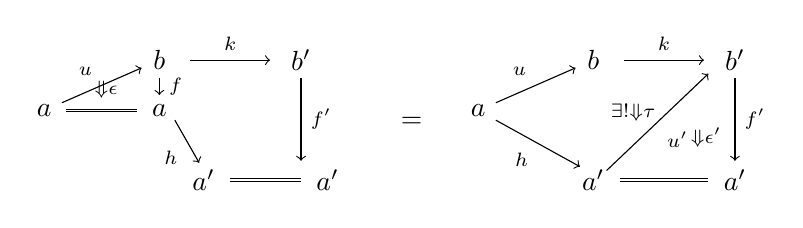
\begin{tikzpicture}[x=1.6em,y=1.4em]
  \node (al) at (0,1.2)     {$a$};
  \node (bl) at (2.6,2.5)   {$b$};
  \node (am) at (2.6,1.2)   {$a$};
  \node (bp) at (5.8,2.5)   {$b'$};
  \node (a1l) at (3.6,-0.6) {$a'$};
  \node (a1m) at (6.4,-0.6) {$a'$};
  \draw[->] (0.4,1.4) -- node[above left]{$\scriptstyle u$} (2.2,2.3);
  \draw[->] (2.6,2.05) -- node[right]{$\scriptstyle f$} (2.6,1.6);
  \draw[double] (0.5,1.2) -- (2.1,1.2);
  \node at (1.4,1.75) {$\scriptstyle\Downarrow\epsilon$};
  \draw[->] (3.3,2.5) -- node[above]{$\scriptstyle k$} (5.1,2.5);
  \draw[->] (2.95,0.95) -- node[below left]{$\scriptstyle h$} (3.5,-0.15);
  \draw[->] (5.8,2.05) -- node[right]{$\scriptstyle f'$} (5.8,-0.1);
  \draw[double] (4.2,-0.6) -- (5.8,-0.6);
  \node at (8.3,0.9) {$=$};
  \node (ar) at (9.8,1.2)    {$a$};
  \node (br) at (12.4,2.5)   {$b$};
  \node (bpr) at (15.6,2.5)  {$b'$};
  \node (a2l) at (12.4,-0.6) {$a'$};
  \node (a2m) at (15.6,-0.6) {$a'$};
  \draw[->] (10.2,1.4) -- node[above left]{$\scriptstyle u$} (12.0,2.3);
  \draw[->] (13.1,2.5) -- node[above]{$\scriptstyle k$} (14.9,2.5);
  \draw[->] (10.2,0.95) -- node[below left]{$\scriptstyle h$} (12.1,-0.25);
  \draw[->] (12.7,-0.35) -- node[below right]{$\scriptstyle u'$} (15.0,2.15);
  \draw[->] (15.6,2.05) -- node[right]{$\scriptstyle f'$} (15.6,-0.1);
  \draw[double] (13.0,-0.6) -- (15.0,-0.6);
  \node at (13.3,1.15) {$\scriptstyle\exists!\Downarrow\tau$};
  \node at (14.95,0.5) {$\scriptstyle\Downarrow\epsilon'$};
\end{tikzpicture}
\end{center}
\end{proof}

\begin{proposition}\label{prop:absolute-right-lifting-representable}
考虑一个 2-\trCategory{} $\mathcal{C}$ 中的 2-\trCell{}
\begin{center}
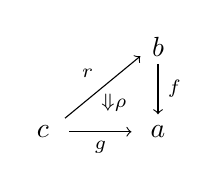
\begin{tikzpicture}[x=1.6em,y=1.4em]
  \node (b) at (2.6,2.2) {$b$};
  \node (c) at (0,0) {$c$};
  \node (a) at (2.6,0) {$a$};
  \draw[->] (0.5,0.35) -- node[above left]{$\scriptstyle r$} (2.2,1.95);
  \draw[->] (2.6,1.75) -- node[right]{$\scriptstyle f$} (2.6,0.45);
  \node at (1.6,0.75) {$\scriptstyle\Downarrow\rho$};
  \draw[->] (0.6,0) -- node[below]{$\scriptstyle g$} (2.0,0);
\end{tikzpicture}
\end{center}
\begin{enumerate}[label=(\roman*)]
\item 若 $(r,\rho)$ 在 $\mathcal{C}$ 中定义一个绝对右\trLifting{}图，则
  \begin{enumerate}[label=(\alph*)]
  \item 对一切 $x\in\mathcal{C}$，
\begin{center}
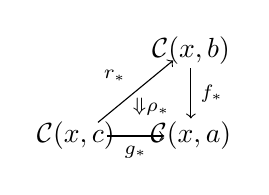
\begin{tikzpicture}[x=1.6em,y=1.4em]
  \node (xb) at (2.6,2.2) {$\mathcal{C}(x,b)$};
  \node (xc) at (0,0) {$\mathcal{C}(x,c)$};
  \node (xa) at (2.6,0) {$\mathcal{C}(x,a)$};
  \draw[->] (0.5,0.35) -- node[above left]{$\scriptstyle r_{\ast}$} (2.2,1.95);
  \draw[->] (2.6,1.75) -- node[right]{$\scriptstyle f_{\ast}$} (2.6,0.45);
  \node at (1.7,0.75) {$\scriptstyle\Downarrow\rho_{\ast}$};
  \draw[->] (0.7,0) -- node[below]{$\scriptstyle g_{\ast}$} (2.0,0);
\end{tikzpicture}
\end{center}
    在 $\Cat$ 中定义一个绝对右\trLifting{}图。
  \item 对一切 $k\colon w\to x\in\mathcal{C}$，所诱导的变换是右正合的。
\begin{center}
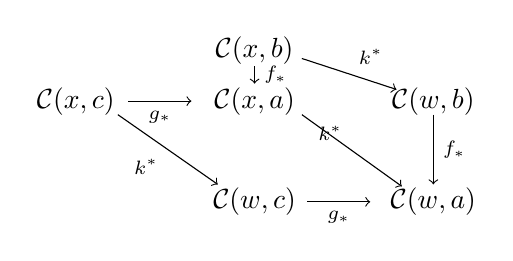
\begin{tikzpicture}[x=1.9em,y=1.4em]
  \node (xcb) at (3.4,2.6) {$\mathcal{C}(x,b)$};
  \node (xcc) at (0,1.3) {$\mathcal{C}(x,c)$};
  \node (xca) at (3.4,1.3) {$\mathcal{C}(x,a)$};
  \node (cwb) at (6.8,1.3) {$\mathcal{C}(w,b)$};
  \node (cwc) at (3.4,-1.3) {$\mathcal{C}(w,c)$};
  \node (cwa) at (6.8,-1.3) {$\mathcal{C}(w,a)$};
  \draw[->] (3.4,2.2) -- node[right]{$\scriptstyle f_{\ast}$} (3.4,1.75);
  \draw[->] (4.3,2.4) -- node[above right]{$\scriptstyle k^{\ast}$} (6.1,1.6);
  \draw[->] (1.0,1.3) -- node[below]{$\scriptstyle g_{\ast}$} (2.2,1.3);
  \draw[->] (0.8,0.95) -- node[below left]{$\scriptstyle k^{\ast}$} (2.7,-0.85);
  \draw[->] (4.3,0.95) -- node[above left]{$\scriptstyle k^{\ast}$} (6.2,-0.9);
  \draw[->] (6.8,0.95) -- node[right]{$\scriptstyle f_{\ast}$} (6.8,-0.85);
  \draw[->] (4.4,-1.3) -- node[below]{$\scriptstyle g_{\ast}$} (5.6,-1.3);
\end{tikzpicture}
\end{center}
  \end{enumerate}
\item 反之，若 ((a)) 对每个 $x\in\mathcal{C}$ 都成立，则 $(r,\rho)$ 在
  $\mathcal{C}$ 中定义一个绝对右\trLifting{}图。
\item 此外，若 $g\colon c\to a$ 与 $f\colon b\to a$ 使得对一切
  $x\in\mathcal{C}$，\trFunctor{} $g_{\ast}\colon\mathcal{C}(x,c)\to\mathcal{C}(x,a)$
  容许一个沿 $f_{\ast}\colon\mathcal{C}(x,b)\to\mathcal{C}(x,a)$ 的绝对右%
  \trLifting{}且条件 ((b)) 对其成立，则 $g$ 在 $\mathcal{C}$ 中容许一个沿 $f$
  的绝对右\trLifting。
\end{enumerate}
\end{proposition}

\begin{proof}
第一个陈述最为直接，我们将其证明留给读者，提示是：为验证 $\Cat$ 中一个绝对%
\trLifting{}图的\trUniversalProperty，只需考虑余跨度 $(g_{\ast},f_{\ast})$
之上以终\trCategory{} $1$ 为顶点的那些\trCone。

对于第二个断言，考虑 $\mathcal{C}$ 中余跨度 $(g,f)$ 之上的一个\trCone
\begin{center}
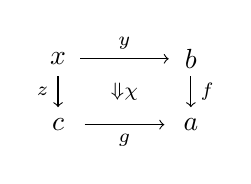
\begin{tikzpicture}[x=1.6em,y=1.4em]
  \node (x) at (0,1.7) {$x$};
  \node (b) at (3.0,1.7) {$b$};
  \node (c) at (0,0) {$c$};
  \node (a) at (3.0,0) {$a$};
  \draw[->] (0.5,1.7) -- node[above]{$\scriptstyle y$} (2.5,1.7);
  \draw[->] (0,1.25) -- node[left]{$\scriptstyle z$} (0,0.45);
  \draw[->] (3.0,1.25) -- node[right]{$\scriptstyle f$} (3.0,0.45);
  \draw[->] (0.6,0) -- node[below]{$\scriptstyle g$} (2.4,0);
  \node at (1.5,0.85) {$\scriptstyle\Downarrow\chi$};
\end{tikzpicture}
\end{center}
这份数据定义了如下图左侧所示的一个\trCategory{}图表，它唯一地分解成右侧所示的
形状：
\begin{center}
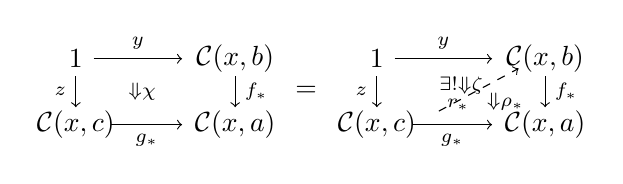
\begin{tikzpicture}[x=1.6em,y=1.4em]
  \node (one) at (0,1.7) {$1$};
  \node (cxb) at (3.6,1.7) {$\mathcal{C}(x,b)$};
  \node (cxc) at (0,0) {$\mathcal{C}(x,c)$};
  \node (cxa) at (3.6,0) {$\mathcal{C}(x,a)$};
  \draw[->] (0.4,1.7) -- node[above]{$\scriptstyle y$} (2.4,1.7);
  \draw[->] (0,1.25) -- node[left]{$\scriptstyle z$} (0,0.45);
  \draw[->] (3.6,1.25) -- node[right]{$\scriptstyle f_{\ast}$} (3.6,0.45);
  \draw[->] (0.8,0) -- node[below]{$\scriptstyle g_{\ast}$} (2.4,0);
  \node at (1.5,0.85) {$\scriptstyle\Downarrow\chi$};
  \node at (5.2,0.85) {$=$};
  \node (one2) at (6.8,1.7) {$1$};
  \node (cxb2) at (10.6,1.7) {$\mathcal{C}(x,b)$};
  \node (cxc2) at (6.8,0) {$\mathcal{C}(x,c)$};
  \node (cxa2) at (10.6,0) {$\mathcal{C}(x,a)$};
  \draw[->] (7.2,1.7) -- node[above]{$\scriptstyle y$} (9.4,1.7);
  \draw[->] (6.8,1.25) -- node[left]{$\scriptstyle z$} (6.8,0.45);
  \draw[->] (10.6,1.25) -- node[right]{$\scriptstyle f_{\ast}$} (10.6,0.45);
  \draw[->] (7.6,0) -- node[below]{$\scriptstyle g_{\ast}$} (9.4,0);
  \node at (8.7,1.0) {$\scriptstyle\exists!\Downarrow\zeta$};
  \draw[->,dashed] (8.2,0.35) -- node[below left]{$\scriptstyle r_{\ast}$} (10.0,1.45);
  \node at (9.7,0.6) {$\scriptstyle\Downarrow\rho_{\ast}$};
\end{tikzpicture}
\end{center}
从而定义出所求的唯一分解
\begin{center}
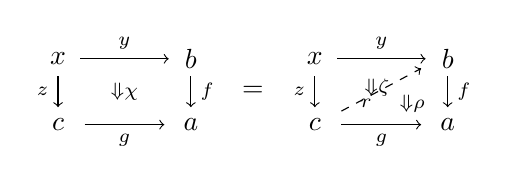
\begin{tikzpicture}[x=1.6em,y=1.4em]
  \node (x) at (0,1.7) {$x$};
  \node (b) at (3.0,1.7) {$b$};
  \node (c) at (0,0) {$c$};
  \node (a) at (3.0,0) {$a$};
  \draw[->] (0.5,1.7) -- node[above]{$\scriptstyle y$} (2.5,1.7);
  \draw[->] (0,1.25) -- node[left]{$\scriptstyle z$} (0,0.45);
  \draw[->] (3.0,1.25) -- node[right]{$\scriptstyle f$} (3.0,0.45);
  \draw[->] (0.6,0) -- node[below]{$\scriptstyle g$} (2.4,0);
  \node at (1.5,0.85) {$\scriptstyle\Downarrow\chi$};
  \node at (4.4,0.85) {$=$};
  \node (x2) at (5.8,1.7) {$x$};
  \node (b2) at (8.8,1.7) {$b$};
  \node (c2) at (5.8,0) {$c$};
  \node (a2) at (8.8,0) {$a$};
  \draw[->] (6.3,1.7) -- node[above]{$\scriptstyle y$} (8.3,1.7);
  \draw[->] (5.8,1.25) -- node[left]{$\scriptstyle z$} (5.8,0.45);
  \draw[->] (8.8,1.25) -- node[right]{$\scriptstyle f$} (8.8,0.45);
  \draw[->] (6.4,0) -- node[below]{$\scriptstyle g$} (8.2,0);
  \node at (7.2,0.95) {$\scriptstyle\Downarrow\zeta$};
  \draw[->,dashed] (6.4,0.35) -- node[below left]{$\scriptstyle r$} (8.2,1.45);
  \node at (8.0,0.55) {$\scriptstyle\Downarrow\rho$};
\end{tikzpicture}
\end{center}
对于最后一个断言，我们把 $(r,\rho)$ 定义为：将所假定的绝对右\trLifting{}
$(r^{c},\rho^{c})$ 的那个\trFunctor{}与那个\trNaturalTransformation{}在情形
$x=c$ 之下于 $\mathrm{id}_{c}\in\mathcal{C}(c,c)$ 处求值。为验证
$\rho\colon fr\Rightarrow g$ 定义 $g$ 沿 $f$ 的一个绝对右\trLifting，考虑一支
1-\trCell{} $z\colon x\to c$。右正合性假设告诉我们，复合变换
\begin{center}
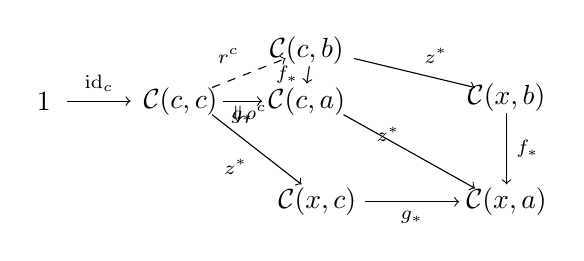
\begin{tikzpicture}[x=1.9em,y=1.4em]
  \node (ccb) at (5.0,2.6) {$\mathcal{C}(c,b)$};
  \node (one) at (0,1.3) {$1$};
  \node (ccc) at (2.6,1.3) {$\mathcal{C}(c,c)$};
  \node (cca) at (5.0,1.3) {$\mathcal{C}(c,a)$};
  \node (cxb) at (8.8,1.4) {$\mathcal{C}(x,b)$};
  \node (cxc) at (5.2,-1.3) {$\mathcal{C}(x,c)$};
  \node (cxa) at (8.8,-1.3) {$\mathcal{C}(x,a)$};
  \draw[->] (0.45,1.3) -- node[above]{$\scriptstyle\mathrm{id}_{c}$} (1.65,1.3);
  \draw[->,dashed] (3.2,1.65) -- node[above left]{$\scriptstyle r^{c}$} (4.6,2.4);
  \node at (3.9,0.95) {$\scriptstyle\Downarrow\rho^{c}$};
  \draw[->] (5.05,2.2) -- node[left]{$\scriptstyle f_{\ast}$} (5.0,1.75);
  \draw[->] (5.9,2.4) -- node[above right]{$\scriptstyle z^{\ast}$} (8.2,1.65);
  \draw[->] (3.4,1.3) -- node[below]{$\scriptstyle g_{\ast}$} (4.15,1.3);
  \draw[->] (8.8,1.0) -- node[right]{$\scriptstyle f_{\ast}$} (8.8,-0.85);
  \draw[->] (3.2,0.95) -- node[below left]{$\scriptstyle z^{\ast}$} (4.9,-0.85);
  \draw[->] (5.7,0.95) -- node[above left]{$\scriptstyle z^{\ast}$} (8.2,-0.95);
  \draw[->] (6.1,-1.3) -- node[below]{$\scriptstyle g_{\ast}$} (7.9,-1.3);
\end{tikzpicture}
\end{center}
是绝对右\trLifting。由上文第二个断言的证明，这告诉我们 $(r^{c},\rho^{c})$ 是
$g_{\ast}$ 沿 $f_{\ast}$ 的一个绝对右\trLifting，从而证得 $(r,\rho)$ 如所求地
是一个绝对右\trLifting。
\end{proof}

\begin{remark}\label{rem:yoneda-perspective}
\cref{prop:adjunctions-representably-defined}与
\cref{prop:absolute-right-lifting-representable}的结果可视为\trBicategorical{} Yoneda
引理的一些应用，后者定义了从\trBicategory{} $\mathcal{C}$ 到由伪函子、伪自然变换与%
\trModification{}组成的 2-\trCategory{} $[\mathcal{C}^{\mathrm{op}},\Cat]$ 的一个%
2-\trFullyFaithful{}嵌入（见第 10 章中的\cref{def:pseudofunctor}、第 10 章中
的\cref{def:pseudonatural-transformation}与附录 B 中的\cref{def:modification}）。
若 $\mathcal{C}$ 中的一支 1-\trCell{} $u\colon a\to b$ 满足%
\cref{prop:adjunctions-representably-defined}的条件 (i)，则由附录 B 中的%
\cref{thm:mates-double-functoriality}，诸\trLeftAdjoint{}
$f^{x}\colon\mathcal{C}(x,b)\to\mathcal{C}(x,a)$ 定义一个%
\trOplax\trNaturalTransformation{}的诸分量。条件 (ii) 要求这个%
\trOplax\trNaturalTransformation{}是一个伪自然变换。如今，2-全忠实性使我们
能把这一点提升为 $\mathcal{C}$ 中的一支箭头 $f\colon b\to a$，后者是 $u$ 的%
\trLeftAdjoint。

至于\cref{prop:equivalences-representably-defined}的情形——其中
$u\colon a\to b$ 诱导诸\trEquivalence{}
$\mathcal{C}(x,a)\Rightarrow\mathcal{C}(x,b)$——诸逆可以经选取而定义%
\trAdjointEquivalence，后者自动地拼装成一个伪自然变换（见第 10 章中的%
\cref{lem:adjoint-inverses-qpn}）。这正是无需任何附加假设的原因。
\end{remark}

\subsection*{练习}

\begin{exercise}\label{ex:confirm-mate-assertion}
确证\cref{lem:mate-right-exact}的证明中所述的论断。
\end{exercise}

\begin{exercise}\label{ex:prove-representable-absolute-lifting}
证明\cref{prop:absolute-right-lifting-representable}(i)。
\end{exercise}

